\documentclass{article}
\usepackage{iclr2027_conference,times}
\input{math_commands.tex}
\usepackage{hyperref}
\usepackage{url}
\usepackage{graphicx}
\usepackage{booktabs}
\usepackage{amsmath,amssymb}

% ---------------------------------------------------------------------------------------------
% HOW TO USE THIS FILE
%  * Upload the whole paper/ folder to Overleaf (New Project -> Upload Project) and compile main.tex.
%  * Do NOT touch margins, fonts or the .sty file: format violations are desk-rejected.
%  * Do NOT uncomment \iclrfinalcopy: leaving it commented keeps the paper anonymous.
%  * Every "TODO" must be gone before submission. Every number must come from paper/tables/*.tex
%    or a results/*.json file (rerun `python plot.py`), never typed from memory.
%  * Citations: lines marked "% CITE:" name the arXiv id to cite. Export the BibTeX yourself from
%    the arXiv/DBLP/Semantic Scholar page into references.bib, read the paper, then add \citep{key}.
%    Never cite a paper you have not opened.
%  * Main text limit: 9 pages. References, the statements at the end and the appendix do not count.
% ---------------------------------------------------------------------------------------------

\title{Do GLU Gates Need Full Rank? An Asymmetry Study of Transformer Feed-Forward Blocks}

\author{Anonymous authors \\ Paper under double-blind review}

\newcommand{\fix}{\marginpar{FIX}}
\newcommand{\new}{\marginpar{NEW}}
\newcommand{\todo}[1]{\textcolor{red}{[TODO: #1]}}
\usepackage{xcolor}

%\iclrfinalcopy
\begin{document}
\maketitle

\begin{abstract}
% SEP 18 VERSION (no results yet). Replace with the full version from the plan once numbers exist.
Gated linear units (GLUs) are the standard feed-forward block in modern Transformers and spend three
equally sized projections per block: a gate, an up-projection, and a down-projection. These play
different roles: the gate selects which hidden units are active, while the up- and down-projections
carry the content written back to the residual stream. Standard architectures nevertheless give all
three the same capacity. We ask whether selection is cheaper than content.
First, in a training-free study of open pretrained language models, we compare truncating each
projection to the same rank at matched parameter savings, using both plain and activation-aware
singular value decompositions. Second, we study the thin-gate GLU, which factorizes only the gate
through a low-rank bottleneck and leaves the content path dense, and evaluate it against dense,
width-reduced, and uniformly low-rank baselines, as well as the symmetric controls that factorize only
the up- or only the down-projection, in small-scale language-model pretraining with multiple seeds.
Third, we test whether pretrained models can be converted by truncating one projection and training only
the new factors. We report measured throughput and memory alongside parameter and FLOP counts, and
discuss the limited scale of our experiments.
\end{abstract}

\section{Introduction}
% Write this LAST, from the results. Skeleton (one paragraph each):
%  1. GLU FFNs hold ~2/3 of Transformer parameters; all three matrices get equal size by convention.
%  2. Selection vs content: the gate decides which units fire; up/down carry what is written.
%     Related evidence: sparsity predictors are low-rank (CITE Deja Vu line); attention selection is
%     low-dimensional (CITE: arXiv 2603.04427).
%  3. Gap: low-rank FFN training factorizes all matrices uniformly (CITE: arXiv 2406.16450, 2407.09835);
%     nobody isolates the gate. \todo{confirm with a literature search; soften if you find prior work}
%  4. What we do (A, B, C) and what we find. State scale limits HERE, not only in Limitations.
%  5. Contributions as 3 bullets, each one a claim a table/figure directly supports.
\todo{introduction}

\section{Background and Related Work}
\todo{Build from related.md. Groups: (i) GLU variants; (ii) low-rank / structured FFN pretraining;
(iii) post-hoc SVD compression with activation-aware whitening and per-module rank allocation;
(iv) contextual sparsity predictors; (v) selection-vs-content asymmetry in attention.}

\section{Method}
\label{sec:method}

\paragraph{GLU feed-forward block.} For an input $\vx \in \R^{d}$, a SwiGLU block with hidden width
$d_{\mathrm{ff}}$ computes
\begin{equation}
  \mathrm{FFN}(\vx) = \mW_{\mathrm{down}} \big( \sigma(\mW_{\mathrm{gate}} \vx) \odot (\mW_{\mathrm{up}} \vx) \big),
\end{equation}
with $\mW_{\mathrm{gate}}, \mW_{\mathrm{up}} \in \R^{d_{\mathrm{ff}} \times d}$,
$\mW_{\mathrm{down}} \in \R^{d \times d_{\mathrm{ff}}}$, and $\sigma$ the SiLU function. All three matrices
have $d \, d_{\mathrm{ff}}$ parameters.

\paragraph{Thin-gate GLU.} We replace only the gate by a rank-$r$ factorization,
$\mW_{\mathrm{gate}} = \mB \mA$ with $\mA \in \R^{r \times d}$ and $\mB \in \R^{d_{\mathrm{ff}} \times r}$,
and keep $\mW_{\mathrm{up}}$ and $\mW_{\mathrm{down}}$ dense. The gate then costs $r(d + d_{\mathrm{ff}})$
parameters (and multiply-accumulates per token) instead of $d\,d_{\mathrm{ff}}$, so the block shrinks from
$3 d\, d_{\mathrm{ff}}$ to $2 d\, d_{\mathrm{ff}} + r (d + d_{\mathrm{ff}})$. No nonlinearity is inserted between
$\mA$ and $\mB$. Both factors are initialised from a zero-mean normal distribution with standard deviation
$(s^2 / r)^{1/4}$, so that the entries of $\mB\mA$ have the same variance $s^2$ as the dense initialisation.

\paragraph{Controls.} \emph{Thin-up} and \emph{thin-down} apply the same rank-$r$ factorization to
$\mW_{\mathrm{up}}$ or $\mW_{\mathrm{down}}$ instead; because the three matrices have the same shape these
controls have exactly the same parameter count as thin-gate. \emph{Shrunk} is a dense GLU with reduced
$d_{\mathrm{ff}}$; \emph{all-low-rank} factorizes all three matrices at one rank; both are matched to the
thin-gate parameter count (within \todo{x}\%). \emph{Reinvest} is a thin-gate GLU whose $d_{\mathrm{ff}}$ is
widened until it matches the dense parameter count.

\paragraph{Training-free truncation.} For a pretrained model we replace one projection type in every layer by
its best rank-$r$ approximation and measure perplexity. \emph{Plain} truncation uses the SVD of $\mW$.
\emph{Activation-aware} truncation minimises $\|(\mW - \mW')\mX\|_F$ over calibration inputs $\mX$: with the
Cholesky factor $\mS\mS^\top = \mX\mX^\top$ we truncate the SVD of $\mW\mS$ and multiply by $\mS^{-1}$.
% CITE the whitening SVD-compression papers you actually read (e.g. SVD-LLM, ASVD).

\section{Experiments}
\subsection{Setup}
\todo{Models, data (FineWeb GPT-2 tokens; wikitext-2 test for perplexity), token budgets, optimizer, learning
rate and how it was chosen (same sweep for every arm), seeds, hardware (one consumer GPU with 8\,GB).
Full hyperparameters go in the appendix.}

\subsection{Which projection tolerates rank reduction in pretrained models?}
\todo{Figure~\ref{fig:posthoc}; tables/posthoc\_plain.tex and tables/posthoc\_whiten.tex.}
\begin{figure}[h]
  \centering
  % 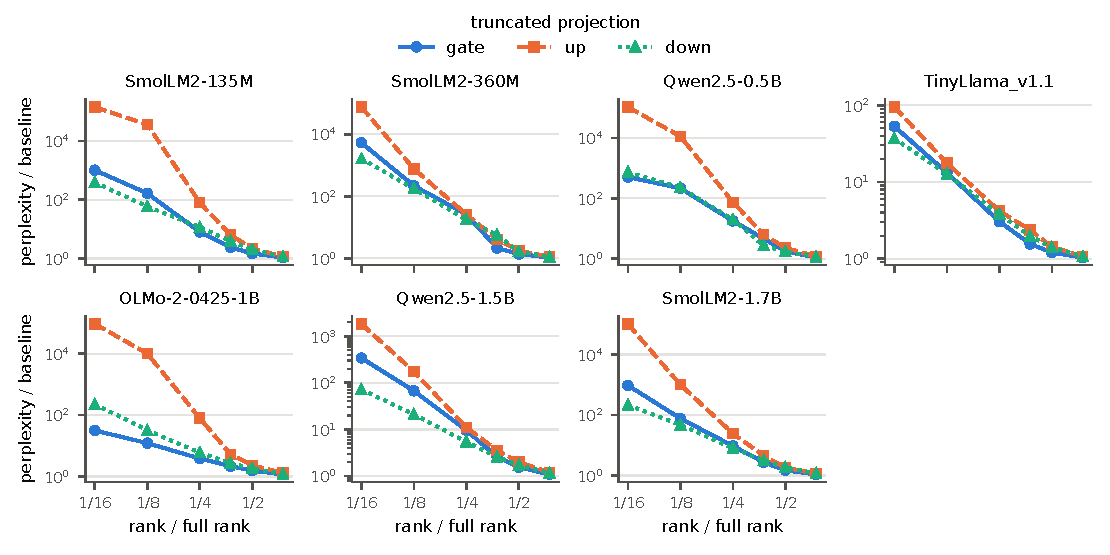
\includegraphics[width=\linewidth]{figures/posthoc_whiten.pdf}
  \caption{\todo{caption: what is plotted, how to read it, the one-sentence takeaway}}
  \label{fig:posthoc}
\end{figure}

\subsection{Pretraining from scratch}
\todo{Figure with figures/training.pdf and tables/training.tex. Report mean $\pm$ std over seeds and compare
every gap to the seed-to-seed spread of the dense baseline. State measured tokens/s, not only FLOPs.}

\subsection{Converting pretrained models}
\todo{tables/heal.tex}

\section{Limitations}
\todo{Scale ($\le$ \todo{P}M parameters, $\le$ \todo{T} tokens, one GPU); short training relative to
production models; one tokenizer and dataset for pretraining; perplexity-centred evaluation; low-rank
matmuls may not be faster at these sizes; conclusions may not transfer to larger models.}

\section{Conclusion}
\todo{3--4 sentences. Claim only what the tables show.}

% ----------------------------------------------------------------------------------------------
\subsection*{AI use statement}
% REQUIRED by ICLR 2027. EDIT THIS so that every sentence is true for what you actually did.
In this work, we used generative AI tools (a large language model assistant) to propose and refine the
research hypothesis, to design and provide feedback on the experimental methodology, to implement the
methods, data-preparation and evaluation code, to clean and reformat the evaluation data, and to help
interpret results. We have not used generative AI tools to generate synthetic data sets, to develop
theoretical models or conceptual frameworks, to formulate mathematical claims, to provide critical
ingredients for proving mathematical claims or to assist in the writing of proofs, to assist with
translation, or to support qualitative or thematic data analysis.
Additionally, we used generative AI tools for brainstorming, searching for and identifying related
literature, suggesting experimental parameters, creating software code and figures, drafting and editing
parts of this paper, and proposing the title.
% VERIFY BEFORE SUBMISSION. Every clause of the next sentence must be true on the day you submit:
%   (1) tests.py passes on the machine that produced the reported numbers;
%   (2) every number in the paper came from a results/*.json through plot.py, none typed by hand;
%   (3) you have read the AI-written code you are submitting as your artifact;
%   (4) you have read every paper cited here, in full, BEFORE citing it (related.md boxes ticked);
%   (5) you ran the manual prior-work search yourself.
% Delete any clause you cannot stand behind. An untrue clause here is a Code of Ethics violation.
We have reviewed all AI-assisted work: the correctness tests accompanying our code were run and pass
(exact reconstruction of a dense layer at full rank, parameter and FLOP counts checked against hand
calculations, and a causality check on the model); every number reported in this paper is generated
programmatically from logged result files rather than transcribed; the AI-written code was read and
checked by the authors; every cited work was read by the authors before being cited; and AI-suggested
ideas were checked for prior work through a manual literature search. We take responsibility for the
final content of this work, including text, claims or artifacts produced with the aid of generative AI.

\subsection*{Ethics statement}
% RECOMMENDED by ICLR 2027, page-limit exempt, max 1 page.
This work studies the parameter efficiency of feed-forward layers in language models. It involves no human
subjects, no personal or sensitive data, and no new data collection: every experiment uses publicly available
pretrained models and public text corpora under their respective licences. We see no direct path from this
work to harmful application beyond the general dual-use character of making language models cheaper to run.
Our experiments were deliberately small and ran on a single consumer GPU, which keeps their energy cost low
but also bounds the conclusions we can draw, as we set out in the limitations.

\subsection*{Reproducibility statement}
All architectural details of the thin-gate GLU and of the control arms are given in
Section~\ref{sec:method}, and every hyperparameter -- model sizes, token budgets, optimizer settings,
learning-rate schedule, batch size and random seeds -- is listed in the appendix. The anonymized source code
is included as supplementary material and contains the pretraining, post-hoc truncation, conversion,
benchmarking and plotting scripts together with the correctness tests. Every figure and table in this paper
is generated from logged JSON result files by a single plotting script, so no reported number is transcribed
by hand. All pretrained models and evaluation datasets are publicly available and are identified by their
exact repository names and configurations in the appendix.

\bibliography{references}
\bibliographystyle{iclr2027_conference}

\appendix
\section{Hyperparameters and additional results}
\todo{Table of model sizes and arms (copy from `python grid.py --table`), learning-rate sweep, benchmark table.}

\end{document}
